\documentclass[12pt]{article}
\usepackage[margin=0.5in]{geometry} 
\usepackage{amsmath,amsthm,amssymb,amsfonts, enumitem, fancyhdr, color, comment, graphicx, environ}
\usepackage{course}
\usepackage{cse468-Spring24}
\usepackage{program}
\usepackage{fancybox}
\usepackage{adjustbox}
\usepackage{quantikz}
\usepackage{../bbkey}
\def\SquareOutline{%
\path (0,0) rectangle (1,1);%
}%
\def\Gate#1{\mbox{\textbf{#1}}}
\def\X{\Gate{X}}
\def\Y{\Gate{Y}}
\def\Z{\Gate{Z}}
\def\I{\Gate{I}}
\def\H{\Gate{H}}
\def\QZero{\ket{0}}
\def\QState#1{\ensuremath{\psi_{#1}}}

\def\Obox#1{\Ovalbox{\hbox to 1ex{\vrule width 0pt height 1ex\hss #1\hss}}}
\def\TFMarked#1#2{\ \stackbox[l][m]{\Obox{#1}~\textbf{true}\\\Obox{#2}~\textbf{false}}}
\def\TF{\TFMarked{\relax}{\relax}}
\def\exp#1{\ensuremath{e^{#1}}}
\newcommand{\Blank}[1][1in]{\mbox{\vrule width #1 depth 2pt}\vrule width 0pt height 2.0em}
\def\BlQb{\mbox{\ensuremath{\Blank[4em]\ket{0}+\Blank[4em]\ket{1}}}}
\newcommand{\Blanket}[1][3em]{%
\mbox{\ensuremath{|\,\Blank[#1]\,\rangle}}}

\def\Tall{\vrule width 0pt height 2em depth 0.5em}

\def\SQB#1#2{%
\ensuremath{%
\begin{pmatrix*}[r] #1 \\ #2\end{pmatrix*}}}

\def\SQBB{\SQB{\Blank[2em]}{\Blank[2em]}}

\def\DQB#1#2#3#4{%
\ensuremath{%
\begin{pmatrix*}[r] #1 \\ #2 \\ #3 \\ #4\end{pmatrix*}}}
\def\DQBB{\DQB{\Blank[2em]}{\Blank[2em]}{\Blank[2em]}{\Blank[2em]}}

\def\FactorProof{%
\begin{align*}
\SQB{a}{b} \otimes \SQB{c}{d} &= \DQBB{} \mbox{ (copy this from your \QState{2} answer top of page)}\\
a\cdot c &= \Blank[3em] \\
a\cdot d &= \Blank[3em] \\
b\cdot c &= \Blank[3em] \\
b\cdot d &= \Blank[3em]
\end{align*}
What is the contradiction, if any?
\LeaveSpace{2in}
}

\begin{document}

\begin{assignment}{Exam I}{8 March 2023}{End of class}

{\small {\large \fbox{READ THIS before starting!}}
This exam is open-book, open-notes, open-Internet, but you must do this
work on your own without contact or conversations with any person.
Because this exam is given in a somewhat distributed manner, no questions will be answered, and no clarifications will be given.  State your assumptions and count on us to be fair and flexible, especially if we have been unclear.


Your work must be legible.  Work that is
difficult to read will receive no credit.  There is a blank page at the end
if you want to show extra work there.

There are 118 points available for this exam, but it will only be scored out of 100.  Extra points earned here will count toward your total exam grade, including Exam~II.

You must sign the pledge below for your exam to count.  Any cheating will
cause the students involved to receive an F for this course. Other unpleasant
actions
may be taken.

You must fill in your identifying information correctly.  
}

\begin{center}\large
\begin{tabular}{|c|c|c|} \hline
\multicolumn{3}{|c|}{{\bf Print  clearly} the following information:}  \\ \hline
\multicolumn{3}{|l|}{Name (print clearly):\Tall{}\hbox to 3in{\hss}}  \\ \hline
\multicolumn{3}{|l|}{Student 6-digit ID (print {\it really} clearly):\Tall{}\hbox to 3in{\hss}} \\ \hline
\end{tabular}
\end{center}

{\bf Pledge:} On my honor, I have neither
given nor received any unauthorized aid on this exam.

Signed:  \Blank\Blank\Blank\Blank \\ \hbox to 5em{\hss}(Be 
sure you filled in your information in the box above!)
%
%
%
\clearpage
\begin{enumerate}
\item\Points{20+4} For the \textbf{true}/\textbf{false} questions below, indicate your response by marking an~\textbf{x} in the appropriate box, like this:
\TFMarked{\textbf{x}}{\relax} or \TFMarked{\relax}{\textbf{x}}.  Each is worth 2 points, so there are 4 points of extra credit here. \textbf{Remember that $\equiv$ means equal up to a global phase.}


\begin{itemize}
    \item When an unpolarized photon hits a polarizing filter, that constitutes a measurement of a photon's polarization.~\TF{}
    \item Each of the Pauli matrices (\X, \Y, and \Z) is its own inverse.~\TF{}
    \item The states $\ket{+}=\frac{1}{\sqrt{2}}\SQB{1}{1}$ and $\ket{-}=\frac{1}{\sqrt{2}}\SQB{1}{-1}$ differ only by a global phase.~\TF{}
    \item The states $i\SQB{0}{1}$ and $\SQB{0}{-1}$ differ only by a global phase.~\TF{}
    \item The conjugate transpose of \SQB{1}{i} is $\left(-1\ \  -i\right)$.~\TF{}
    \item For \emph{all} values of $\theta$, $|e^{i\,\theta}|=1$.\TF{}
    \item For the Pauli matrices, $\Gate{X}\Gate{Y}\Gate{Z}\Gate{Z}\Gate{Y}\equiv\Gate{X}$~\TF{}
    \item The state \[\frac{\ket{10}+\ket{11}}{\sqrt{2}}\] is an entangled state.~\TF{}
    \item The state obtained after measuring the left qubit of \[\frac{\ket{00}+\ket{11}}{\sqrt{2}}\] is an entangled state.~\TF{}
    \item The state \[\Gate{CNOT}\left(\frac{\ket{00}+\ket{11}}{\sqrt{2}}\right)\] is an entangled state.~\TF{}
    \item For all states $\ket{\psi}$, $\Gate{X}\Gate{Z}\ket{\psi}\equiv\Gate{Z}\Gate{X}\ket{\psi}$~\TF{}
       \item Following the measurement of a single qubit in the standard basis, the number of possible states of that qubit is uncountably infinite.~\TF{}

\end{itemize}

\clearpage\item\Points{30+2} For each question below, fill in the blank.  Your answer must appear in the provided blank for proper credit.  Write each response in the provided blank space, fully above the dark line.  For example, to express $\frac{i}{\sqrt{3}}$ you would write \Blank{}\hbox to 0pt{\hskip -4em\raisebox{4pt}{$i/\sqrt{3}$}\hss}.  

Each response is worth~2 points, and there are 2 points of extra credit here.
\begin{itemize}
    \item When a qubit is measured in the \X{} basis, it collapses to an \Blank{}state of the Pauli \X{} matrix. Those states are \Blank{} and \Blank{}.
    \item After a quantum bit is measured in the \X{} basis, suppose it is then measured in the standard (\Z{}) basis. The probability of measuring \ket{0} is \Blank[3.5em]{}\% and the probability of measuring \ket{1} is \Blank[3.5em]{}\%.
    \item Recall that the formula for a state $\ket{\psi}$  on the Bloch sphere is
    \[ \ket{\psi} = \cos(\theta/2) + e^{i\,\phi}sin(\theta/2)\]
    Fill in the table using radians for angles:
    \begin{center}
        \begin{tabular}{ccc}
        State & $\theta$ & $\phi$ \\
        \ket{0} & \Blank & \Blank \\
        \ket{+}=\ket{+x} &\Blank & \Blank \\
        \ket{+y} & \Blank & \Blank
        \end{tabular}
    \end{center}
    \item Fill in the blanks below to show the result of the tensor product: \[
    \ket{+}\otimes\ket{+} = \frac{1}{\Blank[2em]} \begin{pmatrix*}[r]
      \Blank[1.5em] \\
      \Blank[1.5em] \\
      \Blank[1.5em] \\
      \Blank[1.5em]
    \end{pmatrix*}
    \]

\end{itemize}
\clearpage\item\Points{30}
%%%
%%%
\long\def\CircProb#1{%
    \item\Points{15} Consider this circuit:
\begin{center}   
    \adjustbox{valign=t,scale=1.5}{\begin{quantikz}
#1
\end{quantikz}}\end{center}

Fill in the column vectors to show your analysis of the states at the indicated positions of the circuit.  The rest of this page is scratch space, but you are \textbf{not required} to show work for this problem.  \textbf{The parts to fill in are on the next page}.
\Continued{}
\Points{3} each:\\
$\ket{\QState{0}}=\DQBB{}$  $\ket{\QState{1}}=\DQBB{}$  $\ket{\QState{2}}=\DQBB{}$

\item \Points{6} \textbf{Either} express \ket{\QState{2}} as the product of two 1-quibit states:

\[\ket{\QState{2}} = \SQBB \otimes \SQBB \]
\textbf{or} complete the proof below to show that it cannot be factored:
\FactorProof{}
}
%%%
%%%
\begin{itemize}


\CircProb{
\lstick{\QZero{}}&\gate{H}\slice{\ket{\QState{0}}} & \ctrl{1}\slice{\ket{\QState{1}}} & \gate{H}\slice{\ket{\QState{2}}}  & \qw\\
\lstick{\QZero{}} &\qw & \targ{} &  \qw    &  \qw}

\CircProb{\lstick{\QZero{}}&\gate{X}\slice{\ket{\QState{0}}} & \ctrl{1}\slice{\ket{\QState{1}}} & \gate{Z}\slice{\ket{\QState{2}}}  & \qw\\
\lstick{\QZero{}} &\gate{Z} & \targ{} &  \gate{X}    &  \qw}
\end{itemize}




\clearpage\item\Points{10} Bloch Sphere Orienteering:  all answers are in the standard basis.  Write each amplitude in the provided blank space, fully above the dark line.  For example, to express $\frac{i}{\sqrt{3}}$ you would write \Blank{}\hbox to 0pt{\hskip -4em\raisebox{4pt}{$i/\sqrt{3}$}\hss}.

Each response is worth 1 point.



\begin{itemize}
    \item We begin at the North pole of the Bloch sphere.
    \item We are in state \BlQb{}.
    \item We rotate about the \Z{} axis $\pi/4$ radians.  We are now at \BlQb{}.
    \item \vline height 2em width0pt We begin again at the North pole.
    \item We experience a \Y{} gate.  We are now at \BlQb{}.
    \item We then experience a \Z{} gate.  We are now at state \BlQb{}.
    \item We finally experience an \H{} gate.  We are now at state \BlQb{}.
\end{itemize}
\LeaveSpace{1in}
\item\Points{10}  Suppose Alice and Bob decide to form a shared key using the BB84 protocol.  The table below shows the bases they will publish along with their observed results.   Recall the correspondence between observed quantum state and bit values:
\begin{BBKey}
\begin{center}
\BBBasis{}
\end{center}
\end{BBKey}
\def\RowU#1#2#3#4{%
\vrule width 0pt depth 0.5em height 1.2em#1 &#2 & #3 & #4 & & & {\vrule width 0pt depth 13pt\small\TF{}}  \\ \hline}
\def\Row#1#2#3{%
\RowU{\STD}{#1}{#2}{#3}}
\def\RowX#1#2#3{%
\RowU{\HDM}{#1}{#2}{#3}}
\Continued{}
Fill in the table below and be sure to put your final answer for grading in the space provided at the bottom of this page.  Note the following:
\begin{description}
  \item[Agreed Bit?]  After publishing their list of bases, what bit (0 or 1), \textbf{IF ANY}, would Alice and Bob each believe they share, assuming they do not believe Eve is present. Leave these boxes blank if they do not believe they share a common bit based on their published bases.
  \item[Eve Detected?] Does this particular row allow detection of Eve if Alice's and Bob's bits from this row are published?
\end{description}

\begin{BBKey}
\begin{center}\Large
\begin{tabular}{c|c||c|c||c|c||c}
\multicolumn{2}{c||}{Alice Sends} & \multicolumn{2}{c||}{Bob Receives}& \multicolumn{2}{c||}{Agreed bit?}&Eve \\
Basis & Obs & Basis & Obs & Alice & Bob & Detected?\\\hline
\RowX{\BBNe}{\HDM}{\BBNe}
\Row{\BBUp}{\STD}{\BBUp}
\RowX{\BBNe}{\HDM}{\BBSe}
\Row{\BBRt}{\STD}{\BBRt}
\Row{\BBUp}{\HDM}{\BBNe}
\Row{\BBUp}{\STD}{\BBUp}\Row{\BBRt}{\HDM}{\BBSe}
\RowX{\BBSe}{\HDM}{\BBSe}
\Row{\BBRt}{\STD}{\BBUp}
\RowX{\BBNe}{\HDM}{\BBNe}

\end{tabular}
\end{center}
\end{BBKey}
\begin{itemize}
    \item Alice believes the shared key is~\Blank[4in]{}
    \item Bob believes the shared key is\ \ ~\Blank[4in]{}
    \item Eve could have been detected in how many rows of your table?~\Blank{}
\end{itemize}

\clearpage\item\Points{12}
Bob was not paying attention during the lecture on quantum teleportation.  After he separated from Alice, he forgot which bit from Alice would require imposition of an \X{} gate on his qubit, and which would require a \Z{} gate.

So consider the classical, 3-qubit teleportation setup, but where Bob is exactly wrong concerning which qubit controls his \X{} gate and which controls his \Z{} gate.  That resulting, incorrect circuit is:

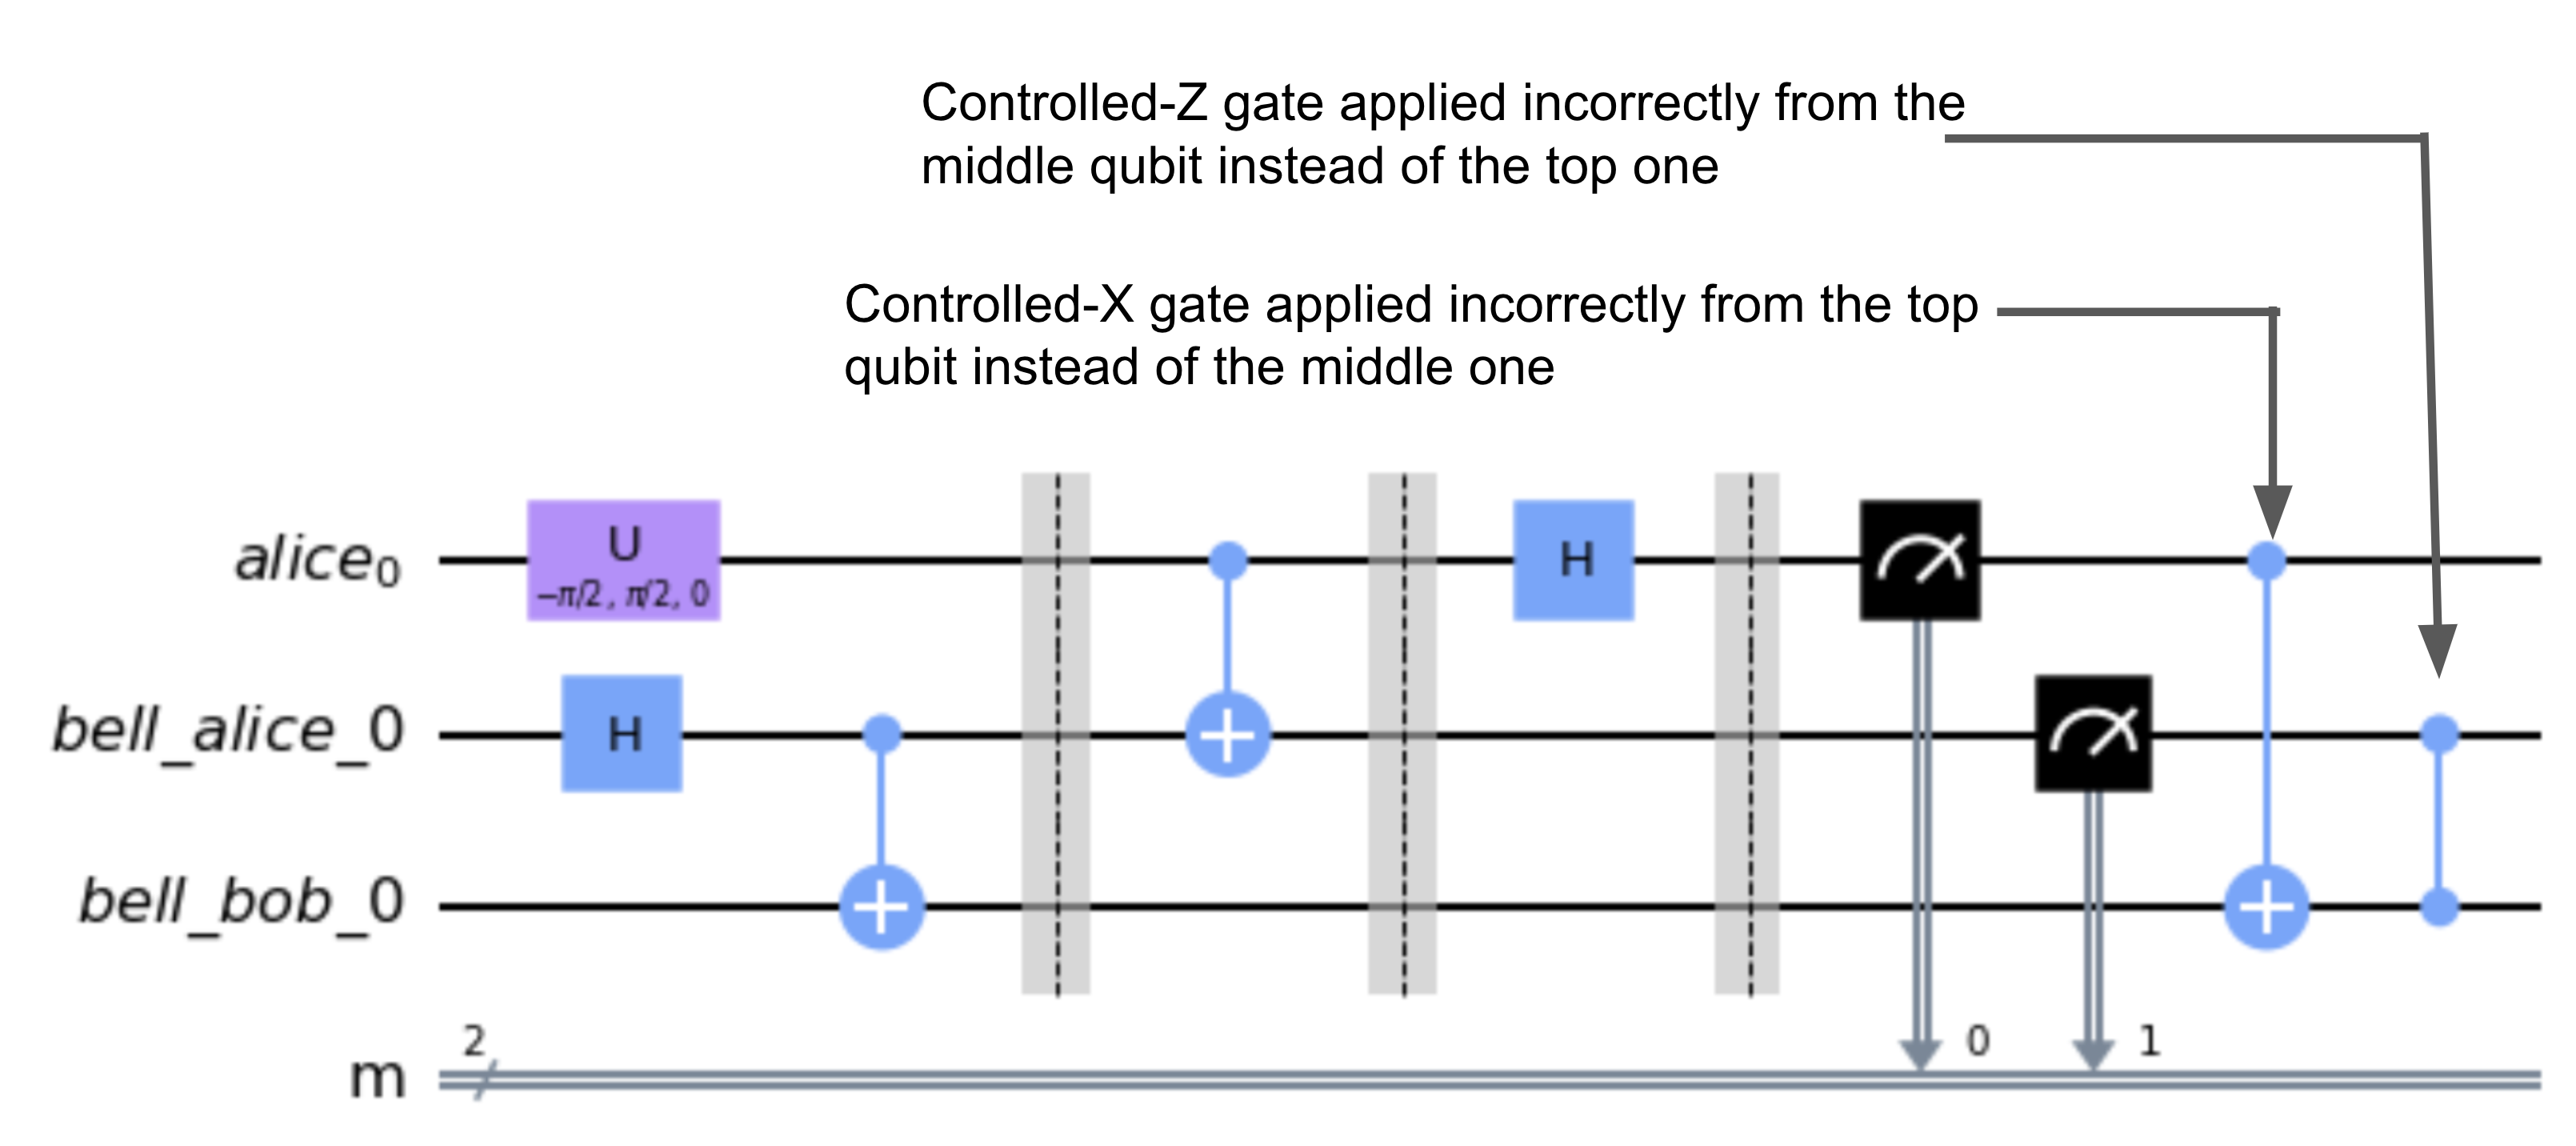
\includegraphics[scale=0.25]{tportwrong.png}

\begin{itemize}
    \item\Points{4}
Complete the table below, \textbf{providing support on the next page}, indicating for which measurements of Alice's qubits, Bob still obtains the correct state on his qubit (\texttt{bell\_bob\_0}).
\begin{center}\Large
\begin{tabular}{ccc}
\multicolumn{2}{c}{Alice's qubit} & Bob obtains the  \\
\texttt{$\mbox{alice}_0$} & \texttt{bell\_alice\_0} & correct state?\\[1em]
0 & 0 & \TF \\[2em]
0 & 1 & \TF \\[2em] 
1 & 0 & \TF \\[2em]
1 & 1 & \TF \\
\end{tabular}
\end{center}
\Continued{}
\item \Points{8} Provide support for your answers here:
\begin{itemize}
    \item \Points{2} Case 00:
    \LeaveSpace{1.5in}
   \item \Points{2} Case 01:
    \LeaveSpace{1.5in}
       \item \Points{2} Case 10:
    \LeaveSpace{1.5in}
       \item \Points{2} Case 11:
    \LeaveSpace{1.5in}
\end{itemize}
\end{itemize}

\end{enumerate}

\end{assignment}
\Bpage{}

\end{document}
